\documentclass[12pt]{exam}
\usepackage{amsmath}
\usepackage{amssymb}
\usepackage{amsthm}
\usepackage{tikz}
\usepackage{mathtools}
\usepackage{graphicx}
\usepackage{wrapfig}

\usepackage{bm} %bold symbols
\usepackage{hyperref} %add links

%%%%%%%%%%%%%%%%%%%%%%%%%
% 	Define vars here 	%
%%%%%%%%%%%%%%%%%%%%%%%%%

\def\hwName{Homework Set 4: §14.1 – 14.5}
\author{Zhengyu James Pan} %use like \@author
\def\email{jzpan@umich.edu}
\makeatletter

\begin{document}
%Header
\pagestyle{head}
\firstpageheader{}{}{}
\header{MATH 215}{\hwName}{\thepage}

%Solution formatting
\printanswers
\unframedsolutions

%Top matter
{\parindent0in
\begin{center}
	\bf MATH 215 FALL 2023\\
	\bf \hwName \\
	\@author\ (\href{mailto:\email}{\email})
\end{center}
}

\begin{questions}
%1
\question Do Exercise 32 of §14.1 of Stewart’s Multivariable Calculus.
\begin{parts}
	\part \boxed{III}--
	\part \boxed{I}--
	\part \boxed{IV}--
	\part \boxed{V}--
	\part \boxed{VI}--
	\part \boxed{II}--
\end{parts}\clearpage
%\clearpage
%2
\question Do Exercises 61-66 of §14.1 of Stewart’s Multivariable Calculus. \\
\textbf{Solutions:}
\begin{questions}
	\setcounter{question}{60}
	\question 
		\begin{parts}
			\part \boxed{C} --very bumpy surface, more bumps with greater x and y
			\part \boxed{II}
		\end{parts}
	\question 
		\begin{parts}
			\part \boxed{A}-- bumpy in y direction
			\part \boxed{IV}
		\end{parts}
	\question 
		\begin{parts}
			\part \boxed{F} --bumps are diagonal, like $y=x$
			\part \boxed{I}
		\end{parts}
	\question 
		\begin{parts}
			\part \boxed{B}
			\part \boxed{VI}
		\end{parts}
	\question 
		\begin{parts}
			\part \boxed{D}
			\part \boxed{V}
		\end{parts}
	\question 
		\begin{parts}
			\part \boxed{D}
			\part \boxed{V}
		\end{parts}
\end{questions}
\setcounter{question}{2}\clearpage
%\clearpage
%3
\question Do Exercise 6 of §14.3 of Stewart’s Multivariable Calculus.
	\begin{solution}
		\begin{align*}
			f_x(2, 1): \\
			f(2, 1) &= 10 \\
			f(2.7, 1) &= 12 \\
			f(1.1, 1) &= 8 \\
			\frac{\delta f(x+)}{\delta x} &= \frac{2}{0.7} = \frac{20}{7} \\
			\frac{\delta f(x-)}{\delta x} &= \frac{2}{0.9} = \frac{20}{9}  \\ 
			f_x(2, 1) &\approx \frac{\frac{20}{7} + \frac{20}{9}}{2} = \boxed{2.53968254} \\ \\ 
			f_y(2, 1): \\
			f(2, 1) &= 10 \\
			f(2, 1.8) &= 8 \\
			f(2, 0) &= 12 \\
			\frac{\Delta f(y+)}{\Delta y} &= \frac{-2}{0.8} = \frac{20}{8} \\
			\frac{\Delta f(y-)}{\Delta y} &= \frac{-2}{1} = 2 \\
			f_y(2, 1) &\approx \frac{-\frac{5}{2} - 2}{2} = \boxed{-2.25}
		\end{align*}
	\end{solution}\clearpage
%\clearpage\clearpage
%4
\question 
	\begin{parts}
		\part Suppose $g(x, y) = \sqrt{9 - 9x^2 - y^2}$. Draw a contour map for $g$ and then sketch the graph of $g$.
			\begin{solution}
				\begin{center}
					\includegraphics*[scale=0.3]{images/04-contour.png}
					\includegraphics*[scale=0.3]{images/04-surface.png}
				\end{center}
			\end{solution}
		\part Draw a contour map of the function $m(x, y) = \frac{x}{(x^2 + 3y^2)}$, showing and labelling several level curves.
			\begin{solution}
				\begin{center}
					\includegraphics*[scale=0.3]{images/04-contourb.png}
				\end{center}
			\end{solution}
	\end{parts}\clearpage
%5
\question 
	\begin{parts}
		\part Use a linear approximation to estimate $(0.99)^3 + (2.01)^3 - 6(0.99)(2.01)$.
			\begin{solution}
				\begin{align*}
					f(1, 2) &= -3 \\
					f_x(x, y) &= 3x^2 + y^3 - 6y \\
					f_x(1, 2) &= -1 \\\\
					f_y (x, y) &= x^3 + 3y^2 - 6x \\
					f_y(1, 2) &= 1 \\\\
					f(1 + \Delta x, 2 + \Delta y) &\approx -3 + (\Delta x) \cdot f_x + (\Delta y) \cdot f_y \\
					f(0.99, 1.99) &\approx -3 + (-0.01) \cdot -1 + 0.01 \cdot (1) \\
					f(0.99, 1.99) &\approx \boxed{-2.98}
				\end{align*}
			\end{solution}
		\part Let $f(x, y) = xe^{y^2} - ye^{x^2}$ and find the equation for the tangent plane to the graph of $f$ at (1, 2).
			\begin{solution}
				\begin{align*}{center}
					\nabla (xe^{y^2} - ye^{x^2} - z) &= \langle xe^{y^2} - 2xye^{x^2}, 2yxe^{y^2} - e^{x^2}, -1 \rangle \\
				\end{align*}
				\begin{equation*}
					\boxed{z = (e^4-4e)x + (4e^4 - e)y + e^4 - 2e}
				\end{equation*}
			\end{solution}
		\part What point on the surface $z = x^2 - y^2$ has a tangent plane parallel to the plane found in the previous part?
		\begin{gather*}
			\nabla (x^2 - y^2 - z) = \langle 2x, 2y, -1 \rangle \\
			\boxed{x = \frac{e^4-4e}{2}} \\
			\boxed{y = \frac{4e^4 - e}{2}}
		\end{gather*}
	\end{parts}\clearpage
%6
\question The wave heights h in the open sea depend on the speed $v$ of the wind and the length of time $t$ that the wind has been blowing at that speed. Values of the function $h = f (v, t)$ are recorded in feet in the following table:
	\begin{center}
		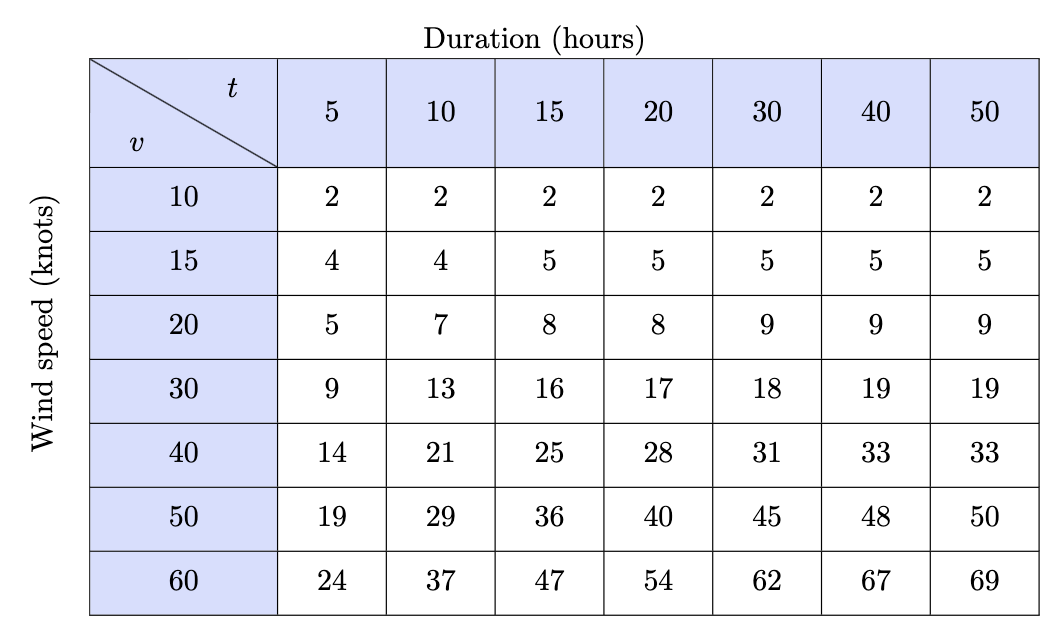
\includegraphics[scale = 0.8]{images/04-table.png}
	\end{center}
	\begin{parts}
		\part What are the meanings of the partial derivatives $\frac{\delta h}{\delta v}$ and $\frac{\delta h}{\delta t}$?
			\begin{solution}
				$\frac{\delta h}{\delta v}$ is the instantaneous rate of change of the wave heights with respect to the speed of the wind. If only the wind speed is changing, this partial derivative determines how much the wave heights are changing. Likewise with $\frac{\delta h}{\delta t}$, the instantaneous rate of change of the wave heights with respect to the time the wind has been blowing at that speed.
			\end{solution}
		\part Estimate the values of $f_v (40, 15)$ and $f_t(40, 15)$. What are the practical interpretations of these values?
			\begin{solution}
				\begin{gather*}
					f_v (40, 15) \approx \frac{(36-25)/10+(25-16)/10}{2} = 1\\
					f_t(40, 15) \approx \frac{(28-25)/5+(25-21)/5}{2} = 0.7
				\end{gather*}
				These are the changes to expect of the wave height if the wind speed and duration were to increase by a single unit, respectively. 
			\end{solution}
		\part Estimate the values of $f_{vv} (30, 20), f_{tt}(30, 20), f_{vt}(30, 20)$, and $f_{tv} (30, 20)$. Are your answers for $f_{tv}$
		the same as for $f_{vt}$? Should they be? Explain. Hint: This problem might be trickier than it looks.
			\begin{solution}
				\begin{gather*}
					f_{tt} (30, 20) \approx \frac{(18-17)/5-(17-16)/5}{5} = 0 \\
					f_{vv}(30, 20) \approx \frac{(28-17)/10-(17-8)/10}{10} = 0.02\\
				\end{gather*}
				\begin{gather*}
					f_{tv} (30, 20) \approx \frac{(f_t(40,20)-f_t(30, 20))/10-(f_t(30, 20) - f_t(20, 20))/10}{10} \\
					\approx \frac{(\frac{(31-28)/10+(28-25)/5}{2}-\frac{(18-17)/10+(17-16)/5}{2})/10-(\frac{(18-17)/10+(17-16)/5}{2} - \frac{(9-8)/10+(8-8)/5}{2})/10}{10} \\
					\approx \boxed{0.002} \\\\
					f_{vt} (30, 20) \approx \frac{(f_v(30,30)-f_v(30, 20))/10-(f_v(30, 20) - f_v(30, 15))/5}{5} \\
					\approx \frac{(\frac{(31-18)/10+(18-9)/10}{2}-\frac{(28-17)/10+(17-8)/10}{2})/10-(\frac{(28-17)/10+(17-8)/5}{2} - \frac{(8-5)/5+(5-2)/5}{2})/5}{5} \\
					\approx \boxed{-0.032}
				\end{gather*}
				The second derivatives need not be equal since we don't necessarily know if Clairaut's theorem applies. 
			\end{solution}
	\end{parts}\clearpage
%7
\question Determine which of the following functions is a solution to Laplace’s equation $u_{xx} + u_{yy} = 0$:
	\begin{parts}
		\part $u(x, y) = \frac{y}{a^2y^2-x^2}$
		\begin{solution}
			\begin{align*}
				u_x &= \dfrac{2yx}{\left(a^2y^2-x^2\right)^2} \\
				u_{xx} &= -\dfrac{2y\cdot\left(3x^2+a^2y^2\right)}{\left(x^2-a^2y^2\right)^3} \\
				u_y &= -\dfrac{a^2y^2+x^2}{\left(a^2y^2-x^2\right)^2} \\
				u_{yy} &= \dfrac{2a^2y\cdot\left(a^2y^2+3x^2\right)}{\left(a^2y^2-x^2\right)^3} \\
				u_{xx} + u_{yy} &\neq 0
			\end{align*}
		\end{solution}
		\part $u(x, y) = x^2 - y^2$
		\begin{solution}
			\begin{align*}
				u_x &= 2x \\
				u_{xx} &= 2 \\
				u_y &= -2y \\
				u_{yy} &= -2 \\
				u_{xx} + u_{yy} &= 0
			\end{align*}
		\end{solution}
		\part $u(x, y) = e^{-x}\cos(y) - e^{-y}\cos x $
		\begin{solution}
			\begin{align*}
				u_x &= \mathrm{e}^{-y}\sin\left(x\right)-\cos\left(y\right)\mathrm{e}^{-x} \\
				u_{xx} &= \mathrm{e}^{-y}\cos\left(x\right)+\cos\left(y\right)\mathrm{e}^{-x} \\
				u_y &= \cos\left(x\right)\mathrm{e}^{-y}-\mathrm{e}^{-x}\sin\left(y\right) \\
				u_{yy} &= -\mathrm{e}^{-x}\cos\left(y\right)-\cos\left(x\right)\mathrm{e}^{-y} \\
				u_{xx} + u_{yy} &= 0
			\end{align*}
		\end{solution}
		\part $u(x, y) = \sin(kx) \sin(aky)$
		\begin{solution}
			\begin{align*}
				u_x &= k\sin\left(aky\right)\cos\left(kx\right) \\
				u_{xx} &= -k^2\sin\left(aky\right)\sin\left(kx\right) \\
				u_y &= ak\sin\left(kx\right)\cos\left(aky\right) \\
				u_{yy} &= -a^2k^2\sin\left(kx\right)\sin\left(aky\right) \\
				u_{xx} + u_{yy} &\neq 0
			\end{align*}
		\end{solution}
		\part $u(x, y) = \ln \sqrt{x^2+y^2}$
		\begin{solution}
			\begin{align*}
				u_x &= \frac{x}{x^2+y^2} \\
				u_{xx} &= \frac{-x^2+y^2}{(x^2+y^2)^2} \\
				u_y &= \frac{y}{y^2+y^2} \\
				u_{yy} &= \frac{-y^2+x^2}{(y^2+y^2)^2} \\
				u_{xx} + u_{yy} &= 0
			\end{align*}
		\end{solution}
	\end{parts}
	\clearpage
%8
\question \begin{parts}
	\part Compute $\lim_{(x,y)→0} f(x, y)$ along an arbitrary straight line path, i.e, along the path $y = ax$, for
	$a \in \mathbf{R}$ some (unknown) constant.
		\begin{solution}
			\begin{gather*}
				f(x, ax) = \frac{ax^2}{1+a^6x^4}\\
				\lim_{(x,y)→0} f(x, ax) = \frac{0}{1+0} = 0
			\end{gather*}
		\end{solution}
	\part Along the curve $y = x^2$, compute $\lim_{(x,y)→0} f(x, y)$
	\begin{solution}
		\begin{gather*}
			f(x, x^2) = \frac{x^7}{x^2 + x^12} = \frac{x^5}{1 + x^10}\\
			\lim_{(x,y)→0} f(x, x^2) = \frac{0}{1+0} = 0
		\end{gather*}
	\end{solution}
	\part Is $f$ continuous at (0, 0)? Explain your reasoning.
	\begin{solution}
		Yes, $f$ seems to be continuous at 0 from the calculations because along arbitrary straight line paths and along a parabolic path, the limit at 0 is 0, which matches the function's value.
	\end{solution}
\end{parts}
\clearpage
%9
\question Consider the function 
	\begin{equation*}
		f(x,y) = 
		\begin{cases}
			\frac{x^3y-xy^3}{x^2+y^2} & \text{ if } (x,y) \neq (0, 0) \\
			0 &\text{ if } (x,y) \neq (0, 0)
		\end{cases}
	\end{equation*}
	\begin{parts}
		\part Based on the plot of the level curves above, does it appear that $f$ is continuous at (0, 0)? Explain.
			\begin{solution}
				No, it does not appear to be continuous because the contour lines are not continued at (0, 0). Thus, it looks like an open point or sudden jump in the function.
			\end{solution}
		\part Find $f_x(x, y)$ and $f_y (x, y)$ when $(x, y) \neq (0, 0)$.
			\begin{solution}
				\begin{align*}
					f_x(x,y) &= \frac{(x^2+y^2)(3x^2y-y^3)-(x^3y-xy^3)(2x)}{(x^2+y^2)^2} \\
					&= \frac{3 x^4 y - x^2 y^3 + 3 x^2 y^3 - y^5 - 2 x^4 y + 2x^2 y^3}{(x^2 + y^2)} \\
					&= \boxed{\frac{x^4y + 4x^2y^3 - y^5}{(x^2+y^2)^2}} \\\\
					f_y(x, y) &= \frac{(x^2+y^2)(x^3-3xy^2)-(x^3y-xy^3)(2y)}{(x^2+y^2)^2} \\
					&= \frac{x^5 - 3 x^3 y^2 + x^3 y^2 - 3 x y^4 - 2 x^3 y^2 + 2 x y^4}{(x^2+y^2)^2} \\
					&= \boxed{\frac{x^5 - 4 x^3 y^2 - x y^4}{(x^2+y^2)^2}}
					\tag*{\qed}
				\end{align*}
			\end{solution}
		\part Can you use your answers from the previous part to find $f_x(0, 0)$ and $f_y (0, 0)$? Explain.
			\begin{solution}
				Yes, since the piecewise $f(0, 0) = 0$ patches the hole in $f$, so we can take the derivative at (0, 0).
			\end{solution}
		\part Using the definition of the partial derivative, find $f_x(0, 0)\text{ and }f_y (0, 0)$.
			\begin{solution}
				\begin{align*}
					f_x (0, 0) &= \displaystyle\lim_{h\rightarrow0} \frac{f(0+h, 0) - f(0,0)}{h} \\
					&= \displaystyle\lim_{h\rightarrow0} \frac{\frac{(x+h)^3y-(x+h)y^3}{(x+h)^2+y^2} - f(0,0)}{h} \\
					&= \displaystyle\lim_{h\rightarrow0} \frac{\frac{0-0}{x^2+2hx+h^2} - 0}{h} \\
					&= \displaystyle\lim_{h\rightarrow0} \frac{\frac{0}{h^2}}{h} \\
					&= \boxed{0}\\\\
					f_y (0, 0) &= \displaystyle\lim_{h\rightarrow0} \frac{f(0,0+h) - f(0,0)}{h} \\
					&= \displaystyle\lim_{h\rightarrow0} \frac{\frac{x^3(y+h)-x(y+h)^3}{x^2+(y+h)^2} - 0}{h} \\
					&= \displaystyle\lim_{h\rightarrow0} \frac{\frac{0}{h^2} - 0}{h}\\ 
					&= \boxed{0}
				\end{align*}
			\end{solution}
		\part Using the definition of the partial derivative, show $f_{xy} (0, 0) = -1\text{ and }f_{yx}(0, 0) = 1$.
			\begin{solution}
				\begin{align*}
					f_{xy} (0, 0) &= \displaystyle\lim_{h\rightarrow0} \frac{f_x(0, 0 + h) - f_x(0,0)}{h} \\
					&= \displaystyle\lim_{h\rightarrow0} \frac{\frac{x^4(y+h) + 4x^2(y+h)^3 - (y+h)^5}{(x^2+(y+h)^2)^2} - f(0,0)}{h} \\
					&= \displaystyle\lim_{h\rightarrow0} \frac{\frac{-h^5 - 0}{h^4} - 0}{h} \\
					&= \boxed{-1}\\\\
					f_{yx} (0, 0) &= \displaystyle\lim_{h\rightarrow0} \frac{f_y(0,0+h) - f_y(0,0)}{h} \\
					&= \displaystyle\lim_{h\rightarrow0} \frac{\frac{(x+h)^5 - 4 (x+h)^3 y^2 - (x+h) y^4}{((x+h)^2+y^2)^2} - 0}{h} \\
					&= \displaystyle\lim_{h\rightarrow0} \frac{\frac{h^5}{h^4} - 0}{h}\\ 
					&= \boxed{1}
				\end{align*}
			\end{solution}
		\part Does the result from the previous part contradiction Clairaut's Theorem? Justify you reasoning.
		Hint: Contour plots, possible generated using something similar to how we plotted a contour from
		MatLab above, might be a way to help bolster your explanation.
			\begin{solution}
				No, this doesn't contradict Clairaut's theorem because the function for $\neq(0, 0)$ had discontinuities originally, so it wouldn't satisfy Clairaut's theorem.
			\end{solution}

	\end{parts}
\clearpage
\question \begin{solution}
	\begin{gather*}
		\frac{\delta}{\delta t}\sqrt{1+t} = \frac{1}{2\sqrt{1+t}} \\
		\frac{\delta}{\delta t}(2+1/3) = \frac{1}{3} \\
		\frac{\delta T}{\delta x}=4 \\
		\frac{\delta T}{\delta y}=3 \\
		\frac{\delta T(3)}{\delta t}=4 \cdot \frac{1}{2\sqrt{1+3}} + 3 \cdot 1/3 = \boxed{2\ C^\circ}
	\end{gather*}
\end{solution}
\clearpage
\question \begin{parts}
	\part \begin{solution}
		\begin{gather*}
			\frac{\delta^2 z}{\delta r \delta s} = \delta(\frac{\delta z}{\delta x}\frac{\delta x}{\delta s} + \frac{\delta z}{\delta y} \frac{\delta y}{\delta s})/(\delta r) \\
			= \delta(\frac{\delta z}{\delta x} 2s + \frac{\delta z}{\delta y} 2r)/ (\delta r) \\
			= 2s(\frac{\delta^2 z}{\delta x^2}\frac{\delta x}{\delta r} + \frac{\delta z}{\delta x^2}\frac{\delta y}{\delta r})+2r(\frac{\delta^2 z}{\delta y^2}\frac{\delta x}{\delta r} + \frac{\delta z}{\delta y^2}\frac{\delta y}{\delta r}) + 2\frac{\delta z}{\delta y} \\
			= 4rs\frac{\delta^2 z}{\delta x^2} + (4r^2 + 4s^2)\frac{\delta^2 z}{\delta x \delta y} + 4rs(\frac{\delta^2 z}{\delta z^2}) + 2\frac{\delta z}{\delta y}
		\end{gather*}
	\end{solution}
	\part \begin{solution}
		\begin{gather*}
			\frac{\delta z}{\delta r} = \frac{\delta z}{\delta x} \frac{\delta x}{\delta r} + \frac{\delta z}{\delta y} \frac{\delta y}{\delta r}\\
			= \frac{\delta z}{\delta x} \cos \theta + \frac{\delta z}{\delta y} \sin \theta \\\\
			\frac{\delta z}{\delta \theta} = \frac{\delta z}{\delta x} \frac{\delta x}{\delta \theta} + \frac{\delta z}{\delta y} \frac{\delta y}{\delta \theta}\\
			= -\frac{\delta z}{\delta x}r\sin \theta + \frac{\delta z}{\delta y} r \cos \theta\\\\
		\end{gather*}
	\end{solution}
	\part \begin{solution}
		\begin{gather*}
			\frac{\delta z}{\delta r} = \frac{\delta z}{\delta x} \frac{\delta x}{\delta r} + \frac{\delta z}{\delta y} \frac{\delta y}{\delta r}\\
			= \frac{\delta z}{\delta x} \cos \theta + \frac{\delta z}{\delta y} \sin \theta \\\\
			\frac{\delta z}{\delta \theta} = \frac{\delta z}{\delta x} \frac{\delta x}{\delta \theta} + \frac{\delta z}{\delta y} \frac{\delta y}{\delta \theta}\\
			= -\frac{\delta z}{\delta x}r\sin \theta + \frac{\delta z}{\delta y} r \cos \theta\\\\
		\end{gather*}
	\end{solution}
\end{parts}
\end{questions}

\end{document}